\documentclass[a4paper,12pt]{article}
\title{HimalCo project: LMF and dictionaries}
\author{C\'eline Buret}

\usepackage{graphicx}
\usepackage[colorlinks=true]{hyperref}
\usepackage{booktabs}
\usepackage{multirow}
\usepackage{longtable}
\usepackage{listings}
\usepackage{polyglossia}
\usepackage{fullpage}

% API
\newfontfamily\phon[Mapping=tex-text, Ligatures=Common, Scale=MatchLowercase, FakeSlant=0.3]{CharisSIL}
\newcommand{\ipa}[1]{{\phon #1}}
% chinois
\newfontfamily\cn[Mapping=tex-text, Ligatures=Common, Scale=MatchUppercase]{SimSun}
\newcommand{\zh}[1]{{\cn #1}}

\begin{document}
\maketitle
\newpage
\section{What is LMF?}

LMF is an ISO (\textit{International Standard Organisation}) standard of Technical Committee 37 and Sub-Committee 4: ISO-TC37/SC4 24613.\\
This standard is suitable for general and specialised dictionaries, monolingual and multilingual. It describes a formal generic structure indepent of publication supports: from a well-formatted unique lexicographical source, we can obtain a printable form and an electronic form of data.\\
LMF follows a lexicographical approach centered on lemma. It is a two layers model: morphological and semantic.

\pagebreak % packages
LMF model is divided into two main parts: what is called the \textit{core package}, a simple, rigid and mandatory skeleton, which is the heart of the model ; and extensions.

\begin{figure}[h]
\centerline{\fbox{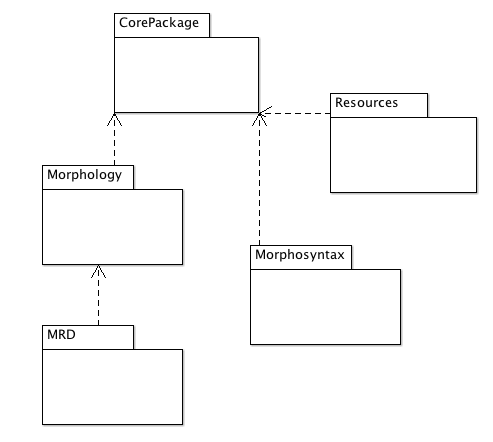
\includegraphics[scale=0.9]{../uml/export/ClassDiagramLMF.png}}}
\caption{LMF packages}
\end{figure}

\pagebreak % Core Package
The \textit{core package} is divided into two sub-systems:
\begin{itemize}
\item the lexical entry, \textit{Lexical Entry}, and its different forms, \textit{Form} (signifier) ;
\item the sens or senses, \textit{Sense} (signified).
\end{itemize}

\begin{figure}[h]
\centerline{\fbox{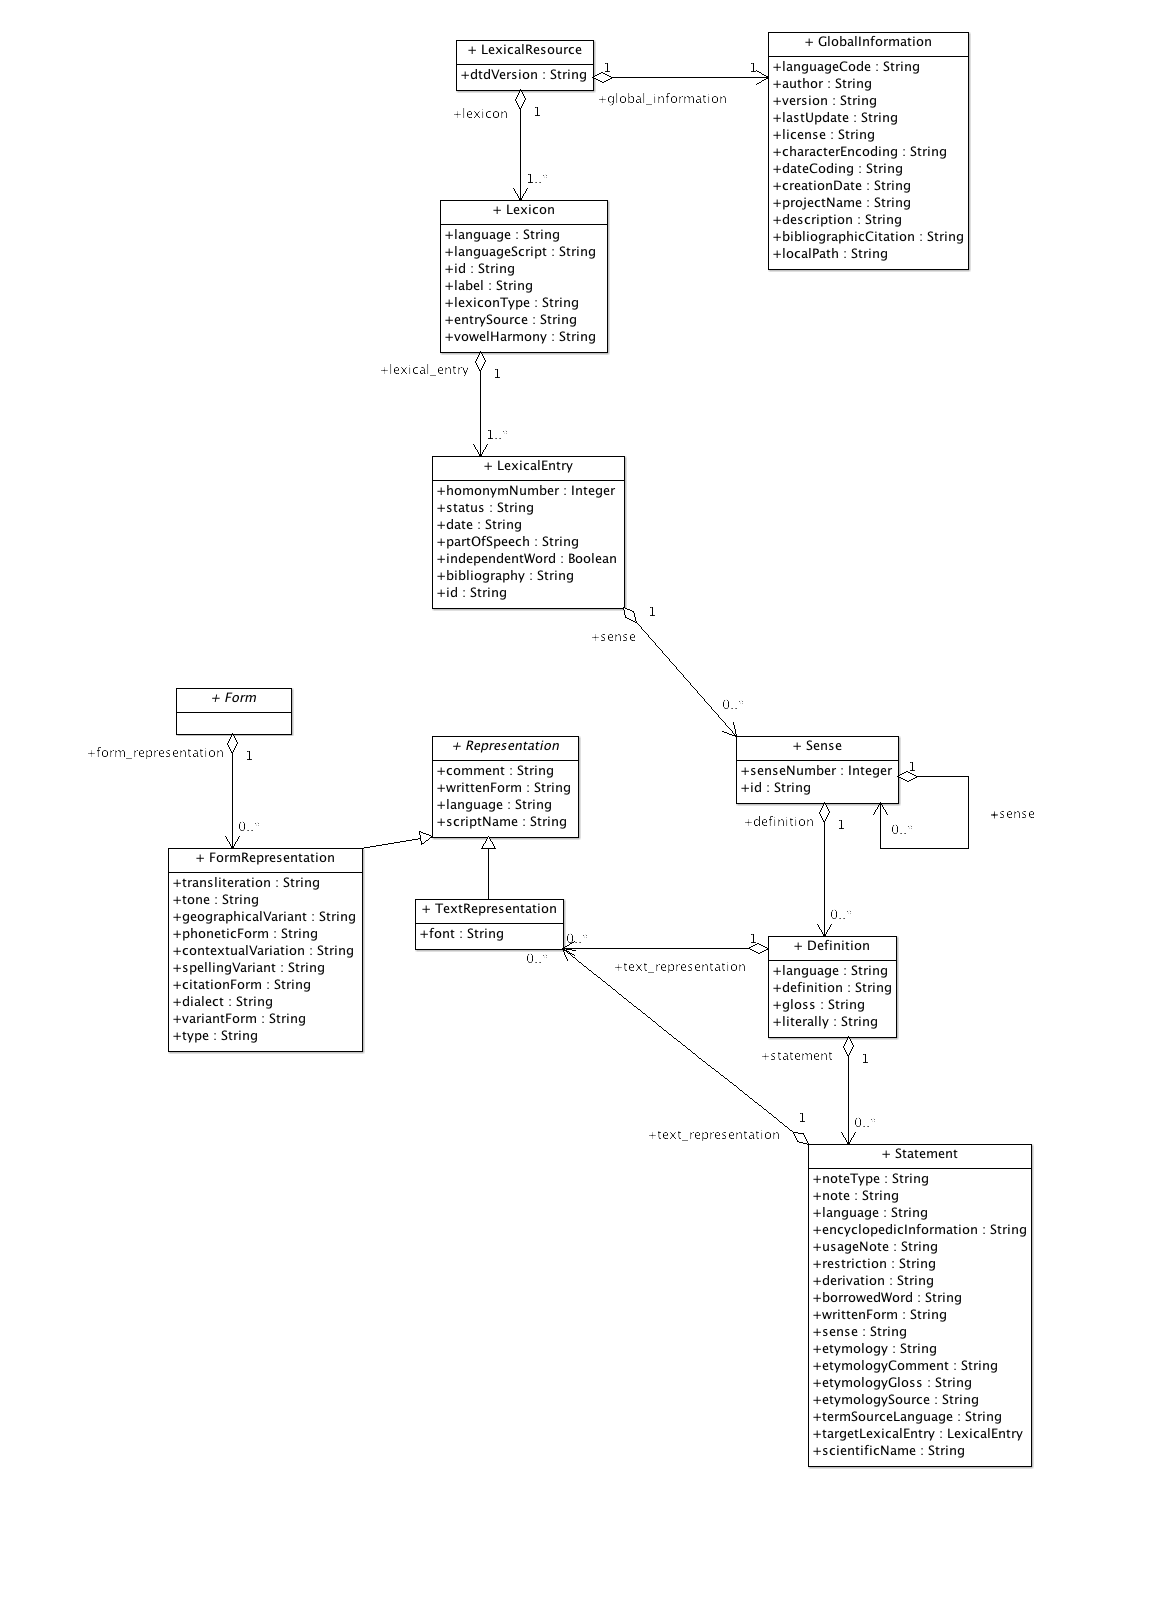
\includegraphics[width=12cm]{../uml/export/ClassDiagramCorePackage.png}}}
\caption{Core Package}
\end{figure}

\pagebreak % existing extensions

Peripheral systems (extensions) are flexible, optional but powerful. Among the 8 proposed extensions, I have selected some that I think are relevant for our needs.

\begin{figure}[h]
\centerline{\fbox{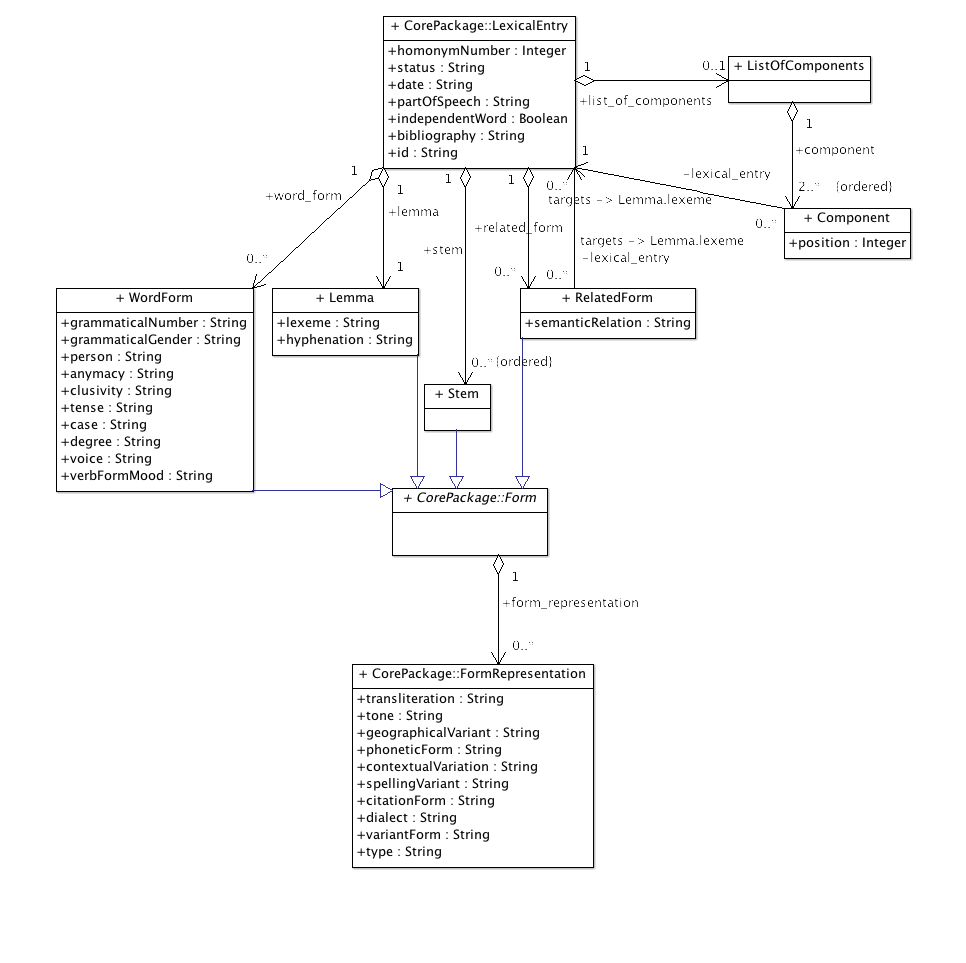
\includegraphics[width=15cm]{../uml/export/ClassDiagramMorphology.png}}}
\caption{Morphology}
\end{figure}
\pagebreak
\begin{figure}[htp]
\centerline{\fbox{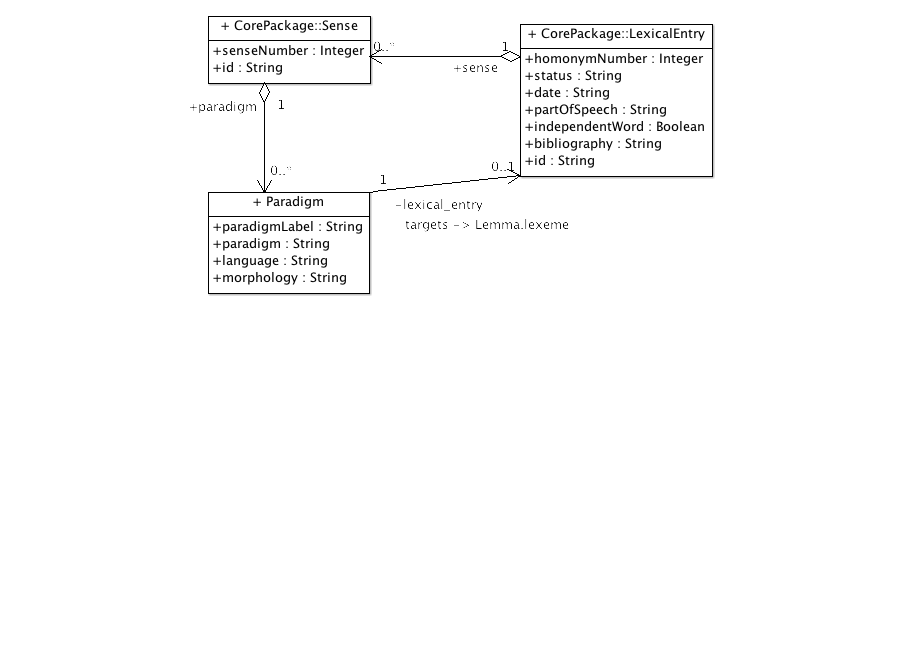
\includegraphics[width=12cm]{../uml/export/ClassDiagramMorphosyntax.png}}}
\caption{Morphosyntax}
\end{figure}
\nopagebreak
\begin{figure}[h]
\centerline{\fbox{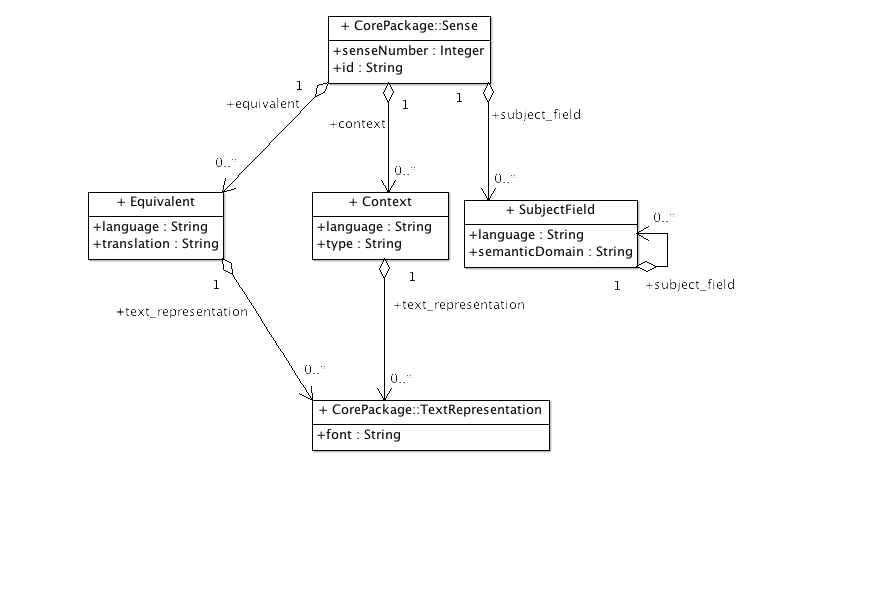
\includegraphics[width=14cm]{../uml/export/ClassDiagramMRD.png}}}
\caption{MRD (Machine Readable Dictionary)}
\end{figure}

\pagebreak % created extensions

In addition to existing extensions, we can create new ones. That is what I propose to do for audio ressources and speakers management.

\begin{figure}[h]
\centerline{\fbox{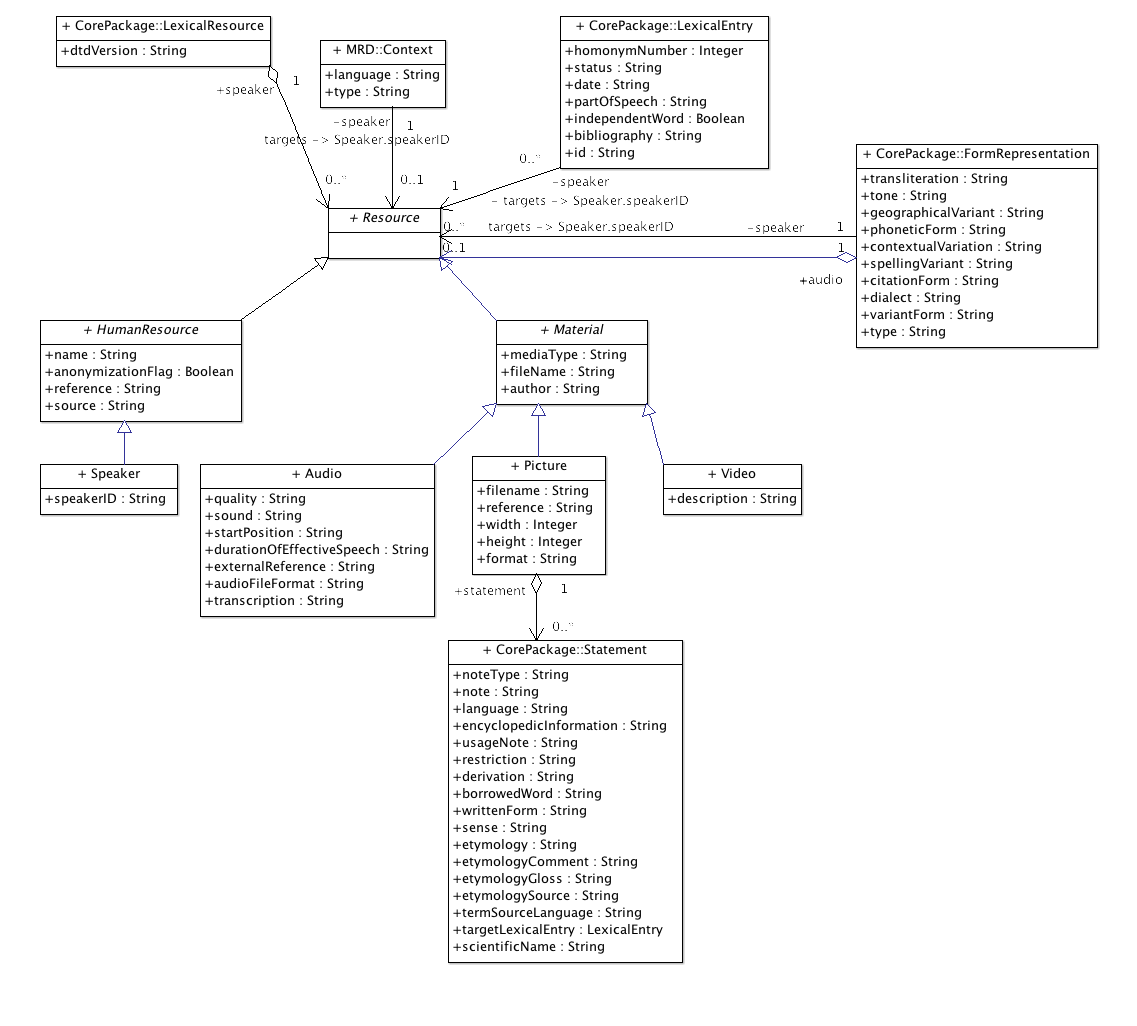
\includegraphics[width=15cm]{../uml/export/ClassDiagramResources.png}}}
\caption{Resources}
\end{figure}

\newpage
\section{Classes and attributes}

In this section, I will focus on what are a class and its attributes - in a simplified way, do not worry. Why? Because there is in fact a direct match between the used software architecture and the chosen XML LMF format.

\subsection{Matching between UML and XML}

A small example in order to have an overview: let us take the \textit{Statement} class of the \textit{Core Package} (at the bottom right of the figure). This class is composed of many attributes, including the 2 following ones:
\begin{itemize}
\item \textit{borrowed word}
\item \textit{written form}
\end{itemize}
By following LMF recommendations, if we wish to represent for instance a borrowing from English of the word \textit{cool} in French, we obtain following XML lines:
\begin{lstlisting}
<Statement>
	<feat att=''borrowed word'' val=''eng''/>
	<feat att=''written form'' val=''cool''/>
</Statement>
\end{lstlisting}
Several comments about this example:
\begin{itemize}
\item In LMF, class attributes are structured as pair of attributes of specific tag \textit{feat}.
\begin{itemize}
\item The name of the attribute is indeed the value of the attribute \textit{att} of the tag \textit{feat} ;
\item The value given to this attribute is the value of the attribute \textit{val} of the tag \textit{feat}.
\end{itemize}
\item In this example, it should be noted that according to LMF (and by the way also MDF), the borrowing language must be filled in the attribute \textit{borrowed word}, while the borrowing word itself is filled in the attribute \textit{written form}.
\end{itemize}

\section{For novices: what is a class?}

A class is an abstract entity that represents an object, for example a car, and that consists of some attributes, for example the brand or the color of the car. A class also has methods, that are functions that it implements: for the car, it would be for example \textit{start}, \textit{accelerate}, etc. Whereas attributes are generally materialized by common names, methods are named by action verbs.\\
On the other hand, a class can inherit from another class, that is, by simplifying, that it inherits from attributes and methods from its mother class. This heritage is represented on preceeding UML schematics by a full arrow. For instance, we could imagine a vehicle class, from which would inherit car, motorcycle, and so on, classes. They would all have common attributes (number of wheels, of doors, brand, color of the vehicle, etc.) that would then be attributes of the vehicle class, and specific attributes as for example the crutch for a motorcycle or a bike.\\
A class can have an aggregation or a compisition relation with another class, i.e. it is part of it. If we take again the basic example of the car and if we create a wheel class, we could say that the car is composed of, among other things, 4 wheels. This relation is represented by a lozenge in UML.\\
Another realtion used in UML schematics of the preceeding section is a simple arrow, which means that a class references another class. For instance, a car and its owner are two distinct entities that exist independantly from each other. However, a link exists between these two entities, represented by an association.\\
At last, in UML, abstract classes are written in italics.

\subsection{Classes and attributes defined in LMF}

For each package described in the previous section, classes and relations between classes are defined and not alterable (note that some existing projects deviate from the standard by proposing enhancements). However, we are (more or less) free to define attributes that we want for each class. But each attribute must be referenced in the DCR (\textit{Data Category Registry}). We can use existing elements, or propose new ones if appropriate. It is an open database, available on the website \url{http://www.isocat.org}.\\
A difficulty that I encountered with this database is that there are a lot of redundancies and duplicates: lots of quite identical terms are defined 2 or 3 times. In this case, which one to choose? According to which criteria? I have tried to focus on the definition that is closest to the need, and at almost similar definition, I have focused on terms issued from MDF, or created by Gil Francopoulo (author of the LMF book). However, rather than follow the MDF principles about markers associated specifically to vernacular, regional and national languages, I have chosen to let more freedom by defining a general attribute associated with a language attribute (example : definition in the 'xxx' language rather than 'dn' that forces a definition in a national predefined language). Moreover, this solution avoids to define for instance 'df' for the French language.\\

In the table below, I have listed attributes of each class, but not methods, because it would weigh down specifications without bringing relevant informations. I have also noted MDF markers which the attributes refer if any. As for concerned LMF extension, it is in the column \textit{LMF package}.

\pagebreak

\begin{center}
\begin{longtable}{*7{p{2cm}}}
\caption[]{LMF classes and their attributes} \\ \hline\hline
\textbf{LMF package} & \textbf{Class name} & \textbf{Attribute} & \textbf{Attribute type or example value} & \textbf{DCR PID and type} & \textbf{MDF marker} & \textbf{Comment} \\ \hline\hline
\endfirsthead
\caption[]{(continued)} \\
\textbf{LMF package} & \textbf{Class name} & \textbf{Attribute} & \textbf{Attribute type or example value} & \textbf{DCR PID and type} & \textbf{MDF marker} & \textbf{Comment} \\
\endhead
\endfoot
\endlastfoot
% CORE PACKAGE
% Lexical Resource
\multirow{82}{2cm}{Core Package} & \multirow{4}{2cm}{Lexical Resource (singleton)} & dtd version & ``16'' & - & - & LMF DTD is an XML attribute \\ \cmidrule{3-7}
& & global information & Global Information & N/A & N/A & \\ \cmidrule{3-7}
& & lexicon & Lexicon & N/A & N/A & \\ \cmidrule{3-7}
& & resource & Speaker & N/A & N/A & \\ \cmidrule{2-7}
% Global Information
& \multirow{11}{2cm}{Global Information (no subclass)} & language code & ``ISO-639-3'' & \href{http://www.isocat.org/datcat/DC-2008}{2008} open & - & \\ \cmidrule{3-7}
& & date coding & ``ISO-8601” & \href{http://www.isocat.org/datcat/DC-2090}{2090} open & - & \\ \cmidrule{3-7}
& & creation date & ``2001-03-24” & \href{http://www.isocat.org/datcat/DC-2510}{2510} open & - & \\ \cmidrule{3-7}
& & last update & ``2014-07-21” & \href{http://www.isocat.org/datcat/DC-2526}{2526} open & - & \\ \cmidrule{3-7}
& & author & ``Alexis Michaud, MICA \& Guillaume Jacques, CRLAO” & \href{http://www.isocat.org/datcat/DC-6130}{6130} open & - & \\ \cmidrule{3-7}
& & version & ``0.1” & \href{http://www.isocat.org/datcat/DC-2547}{2547} open & - & \\ \cmidrule{3-7}
& & license & ``GPL” & \href{http://www.isocat.org/datcat/DC-2457}{2457} open & - & \\ \cmidrule{3-7}
& & project name & ``ANR HimalCo” & \href{http://www.isocat.org/datcat/DC-2536}{2536} open & - & \\ \cmidrule{3-7}
& & description & ``everything you want to tell about this resource” & \href{http://www.isocat.org/datcat/DC-2520}{2520} open & - & \\ \cmidrule{3-7}
& & bibliographic citation & ``Online dictionaries, CNRS, 2014” & \href{http://www.isocat.org/datcat/DC-6137}{6137} open & - & \\ \cmidrule{3-7}
& & character encoding & ``UTF-8” & \href{http://www.isocat.org/datcat/DC-2564}{2564} open & - & \\ \cmidrule{3-7}
% Lexicon
& \multirow{7}{2cm}{Lexicon (no subclass)} & id & ``na?'' & \href{http://www.isocat.org/datcat/DC-1845}{1845} open & - & identifier is an XML attribute (not necessarily unique) \\ \cmidrule{3-7}
& & label & ``Na online dictionary'' & \href{http://www.isocat.org/datcat/DC-1857}{1857} open & - & \\ \cmidrule{3-7}
& & language & ``fra'', ``eng'' & \href{http://www.isocat.org/datcat/DC-2482}{2482} constrained & - & ISO 639 ; vernacular language \\ \cmidrule{3-7}
& & language script & ``latn'' & \href{http://www.isocat.org/datcat/DC-2485}{2485} open & - & ISO 15924 \\ \cmidrule{3-7}
& & lexicon type & ``bilingual dictionary na - eng'' & \href{http://www.isocat.org/datcat/DC-2487}{2487} open & - & \\ \cmidrule{3-7}
& & entry source & ``na\_dic\-tio\-na\-ry.txt'' & \href{http://www.isocat.org/datcat/DC-207}{207} open & - & \\ \cmidrule{3-7}
& & vowel harmony & & no existing DC & - & \\ \cmidrule{3-7}
& & lexical entry & Lexical Entry & N/A & N/A & - \\ \cmidrule{2-7}
% Lexical Entry
& \multirow{16}{2cm}{Lexical Entry (no subclass)} & id & ``toto\_1'' & \href{http://www.isocat.org/datcat/DC-6196}{6196} open & lx \textless id\textgreater, se \textless id\textgreater & unique identifier or key form is an XML attribute \\ \cmidrule{3-7}
& & part of speech (English) & ``verb'' & \href{http://www.isocat.org/datcat/DC-3748}{3748} closed \hyperlink{1}{(1)} \hypertarget{pos}{} & ps & grammatical category \\ \cmidrule{3-7}
& & lemmatized form & Lemma & N/A & N/A & \\ \cmidrule{3-7}
& & date & ``2014-06-15'' & \href{http://www.isocat.org/datcat/DC-3694}{3694} open & dt & \\ \cmidrule{3-7}
& & status & ``no print'', ``done'', ``check'' & \href{http://www.isocat.org/datcat/DC-3760}{3760} open & st & \\ \cmidrule{3-7}
& & homonym number & ``1'' & \href{http://www.isocat.org/datcat/DC-3714}{3714} open & hm & ``0'' if no homonym \\ \cmidrule{3-7}
& & bibliography & ``212'' & \href{http://www.isocat.org/datcat/DC-3687}{3687} open & bb & \\ \cmidrule{3-7}
& & independent word & yes, no & \href{http://www.isocat.org/datcat/DC-5285}{5285} closed & & \\ \cmidrule{3-7}
& & resource & Resource & N/A & N/A & Speaker, Audio, Picture, Video \\ \cmidrule{3-7}
& & form & Form Re\-pre\-sen\-ta\-tion & N/A & N/A & \\ \cmidrule{3-7}
& & sense & Sense & N/A & N/A & \\ \cmidrule{3-7}
& & word form & Word Form & N/A & N/A & \\ \cmidrule{3-7}
& & related form & Related Form & N/A & N/A & \\ \cmidrule{3-7}
& & stem & Stem & N/A & N/A & \\ \cmidrule{3-7}
& & list of components & List Of Components & N/A & N/A & \\ \cmidrule{3-7}
& & borrowed word & Borrowed Word & N/A & N/A & \\ \cmidrule{2-7}
% Form
& \multirow{3}{2cm}{Form (abstract class)} & variant form(s) & ``woman'', ``women'' & \href{http://www.isocat.org/datcat/DC-3768}{3768} open & va, pdl \textless stem\textgreater & written or spoken \\ \cmidrule{3-7}
& & type & \hyperlink{2}{(2)} \hypertarget{type}{} & \href{http://www.isocat.org/datcat/DC-1971}{1971} open & & variant type : spelling, pronunciation, archaic, etc. \\ \cmidrule{3-7}
& & form representation & Form Re\-pre\-sen\-ta\-tion & N/A & N/A & \\ \cmidrule{2-7}
% Form Representation
& \multirow{14}{2cm}{Form Re\-pre\-sen\-ta\-tion} & tone & & \href{http://www.isocat.org/datcat/DC-517}{517} open & np \textless tone\textgreater & \\ \cmidrule{3-7}
& & geographical variant & & \href{http://www.isocat.org/datcat/DC-1851}{1851} open & va & \\ \cmidrule{3-7}
& & phonetic form (vernacular) & & \href{http://www.isocat.org/datcat/DC-3745}{3745} open & ph & \\ \cmidrule{3-7}
& & contextual variation & & \href{http://www.isocat.org/datcat/DC-1977}{1977} open & lc & \\ \cmidrule{3-7}
& & spelling variant & & \href{http://www.isocat.org/datcat/DC-5612}{5612} open & a & \\ \cmidrule{3-7}
& & citation form (vernacular) & & \href{http://www.isocat.org/datcat/DC-3716}{3716} open & lc & \\ \cmidrule{3-7}
& & dialect & ``North German'' & \href{http://www.isocat.org/datcat/DC-2466}{2466} open & ve & \\ \cmidrule{3-7}
& & language & ``fra'', ``eng'' & \href{http://www.isocat.org/datcat/DC-2482}{2482} constrained & - & ISO 639 ; language used for variant comment \\ \cmidrule{3-7}
& & trans\-li\-te\-ra\-tion & ``readable characters'' & \href{http://www.isocat.org/datcat/DC-1848}{1848} open & ph & \\ \cmidrule{3-7}
& & script name & ``Latin'' & \href{http://www.isocat.org/datcat/DC-3809}{3809} open & - & script used for romanization \\ \cmidrule{3-7}
& & resource & Resource & N/A & N/A & Speaker, Video, Picture \\ \cmidrule{3-7}
& & sound & Resource & N/A & N/A & Audio \\ \cmidrule{2-7}
% Representation
& \multirow{3}{2cm}{Re\-pre\-sen\-ta\-tion (abstract class)} & written form & ``...'' & \href{http://www.isocat.org/datcat/DC-1836}{1836} open & xv, xe, xn, xr, xf & example \\ \cmidrule{3-7}
& & language & ``fra'', ``eng'' & \href{http://www.isocat.org/datcat/DC-2482}{2482} constrained & - & ISO 639 ; language used for variant comment \\ \cmidrule{3-7}
& & comment & ``...'' & \href{http://www.isocat.org/datcat/DC-1846}{1846} open & ve, vn, vr, vf, xc & explanation \\ \cmidrule{2-7}
% Text Representation
& \multirow{1}{2cm}{Text Re\-pre\-sen\-ta\-tion} & font & font family / font weight / font size & \href{http://www.isocat.org/datcat/DC-1650}{1650} closed & & 'font-style', 'font-variant', 'line-height' \\ \cmidrule{2-7}
% Sense
& \multirow{9}{2cm}{Sense} & id & ``toto\_1\_1'' & \href{http://www.isocat.org/datcat/DC-1845}{1845} open & - & identifier or key form is an XML attribute (not necessarily unique) \\ \cmidrule{3-7}
& & sense number & ``1'' & \href{http://www.isocat.org/datcat/DC-3758}{3758} open & sn & \\ \cmidrule{3-7}
& & sense & Sense & N/A & N/A & \\ \cmidrule{3-7}
& & definition & Definition & N/A & N/A & \\ \cmidrule{3-7}
& & etymology & Etymology & N/A & N/A & \\ \cmidrule{3-7}
& & paradigm & Paradigm & N/A & N/A & \\ \cmidrule{3-7}
& & equivalent & Equivalent & N/A & N/A & \\ \cmidrule{3-7}
& & context & Context & N/A & N/A & \\ \cmidrule{3-7}
& & subject field & Subject Field & N/A & N/A & \\ \cmidrule{2-7}
% Definition
& \multirow{6}{2cm}{Definition} & definition & ``This is the lexeme definition'' & \href{http://www.isocat.org/datcat/DC-1972}{1972} open & dv, de, dn, dr, df & \\ \cmidrule{3-7}
& & gloss & ``\scshape{GLOSS}'' & \href{http://www.isocat.org/datcat/DC-244}{244} open & gv, ge, gn, gr, gf & \\ \cmidrule{3-7}
& & language & ``fra'', ``eng'' & \href{http://www.isocat.org/datcat/DC-2482}{2482} constrained & - & ISO 639 ; language used for definition and gloss \\ \cmidrule{3-7}
& & literally & 'au pied de la lettre' & \href{http://www.isocat.org/datcat/DC-3721}{3721} open & lt & \\ \cmidrule{3-7}
& & text representation & Text Re\-pre\-sen\-ta\-tion & N/A & N/A & \\ \cmidrule{3-7}
& & statement & Statement & N/A & N/A & \\ \cmidrule{2-7}
% Statement
& \multirow{8}{2cm}{Statement} & note type & \hyperlink{3}{(3)} \hypertarget{nt}{} & \href{http://www.isocat.org/datcat/DC-6178}{6178} open & nt \textless type\textgreater, np \textless type\textgreater, ng \textless type\textgreater & \\ \cmidrule{3-7}
& & note & & \href{http://www.isocat.org/datcat/DC-382}{382} open & na, nd, ng, np, nq, ns, nt & \\ \cmidrule{3-7}
& & language & ``fra'', ``eng'' & \href{http://www.isocat.org/datcat/DC-2482}{2482} constrained & nt \textless lang\textgreater & ISO 639 \\ \cmidrule{3-7}
& & encyclopedic information & ``...'' & \href{http://www.isocat.org/datcat/DC-3828}{3828} open & ee, en, er, ev & \\ \cmidrule{3-7}
& & usage note & ``...'' & \href{http://www.isocat.org/datcat/DC-526}{526} open & uv, ue, un, ur & text \\ \cmidrule{3-7}
& & restriction & ``...'' & \href{http://www.isocat.org/datcat/DC-1956}{1956} open & oe, on, or, ov & \\ \cmidrule{3-7}
& & derivation & ``...'' & \href{http://www.isocat.org/datcat/DC-188}{188} open & - & \\ \cmidrule{3-7}
& & borrowed word (English) & ``Chinese'' & \href{http://www.isocat.org/datcat/DC-3688}{3688} open & bw & source language \\ \cmidrule{3-7}
& & written form & ``...'' & \href{http://www.isocat.org/datcat/DC-1836}{1836} open & bw & loan word \\ \cmidrule{3-7}
& & sense & ``...'' & \href{http://www.isocat.org/datcat/DC-464}{464} open & - & sense in borrowed language \\ \cmidrule{3-7}
& & etymology & ``aspirin: from acetyl + spiraeic acid (old name for salicylic acid)'' & \href{http://www.isocat.org/datcat/DC-221}{221} open & et & \\ \cmidrule{3-7}
& & etymology comment (English) & & \href{http://www.isocat.org/datcat/DC-3696}{3696} open & ec & \\ \cmidrule{3-7}
& & target lexical entry & Lexical Entry & & cf \textless type=''et''\textgreater & \\ \cmidrule{3-7}
& & term source language & ``fra'', ``eng'' & \href{http://www.isocat.org/datcat/DC-3639}{3639} open & - & language \\ \cmidrule{3-7}
& & etymology gloss & & \href{http://www.isocat.org/datcat/DC-3698}{3698} open & eg & \\ \cmidrule{3-7}
& & etymology source & & \href{http://www.isocat.org/datcat/DC-3701}{3701} & es & \\ \cmidrule{3-7}
& & scientific name & ``Canis lupus familiaris'' & \href{http://www.isocat.org/datcat/DC-3754}{3754} open & sc & \\ \cmidrule{3-7}
& & text representation & Text Re\-pre\-sen\-ta\-tion & N/A & N/A & \\ \cmidrule{1-7}
% MORPHOLOGY
% List Of Components
\multirow{18}{2cm}{Morphology} &List Of Components & component & Component & N/A & N/A & \\ \cmidrule{2-7}
% Component
& \multirow{2}{2cm}{Component} & position & ``2'' & \href{http://www.isocat.org/datcat/DC-2183}{2183} open & - & \\ \cmidrule{3-7}
& & target lexical entry & Lexical Entry & N/A & N/A & \\ \cmidrule{2-7}
% Word Form
& \multirow{10}{2cm}{Word Form} & grammatical number & collective, dual, paucal, plural, quadrial, singular, trial & \href{http://www.isocat.org/datcat/DC-1298}{1298} closed & & \\ \cmidrule{3-7}
& & grammatical gender & common gender, feminine, masculine, neuter & \href{http://www.isocat.org/datcat/DC-1297}{1297} closed & & \\ \cmidrule{3-7}
& & person & first person, second person, third person & \href{http://www.isocat.org/datcat/DC-1328}{1328} closed & & \\ \cmidrule{3-7}
& & anymacy & animate, inanimate, other anymacy & \href{http://www.isocat.org/datcat/DC-1902}{1902} closed & & \\ \cmidrule{3-7}
& & clusivity & inclusive, exclusive & \href{http://www.isocat.org/datcat/DC-3031}{3031} closed & & \\ \cmidrule{3-7}
& & tense & future, imperfect, past, present & \href{http://www.isocat.org/datcat/DC-1286}{1286} closed & & \\ \cmidrule{3-7}
& & voice & active voice, middle voice, passive voice & \href{http://www.isocat.org/datcat/DC-1413}{1413} closed & & \\ \cmidrule{3-7}
& & verb form mood & \hyperlink{4}{(4)} \hypertarget{mood}{} & \href{http://www.isocat.org/datcat/DC-1427}{1427} closed & & \\ \cmidrule{3-7}
& & case & ``accusative case'' & \href{http://www.isocat.org/datcat/DC-1840}{1840} closed & & \\ \cmidrule{3-7}
& & degree & comparative degree, positive degree, superlative degree & \href{http://www.isocat.org/datcat/DC-2779}{2779} closed & & \\ \cmidrule{2-7}
% Lemma
& \multirow{2}{2cm}{Lemma} & lexeme & ``toto'' & \href{http://www.isocat.org/datcat/DC-3723}{3723} open & lx & \\ \cmidrule{3-7}
& & hyphenation & ``pho-ne-ti-cian'' & \href{http://www.isocat.org/datcat/DC-264}{264} open & - & syllables separated by '-' \\ \cmidrule{2-7}
% Stem
& \multirow{1}{2cm}{Stem} & & & N/A & N/A & \\ \cmidrule{2-7}
% Related Form
& \multirow{2}{2cm}{Related Form} & semantic relation & \hyperlink{5}{(5)} \hypertarget{relation}{} & \href{http://www.isocat.org/datcat/DC-6331}{6331} open & sy, an, cf \textless et\textgreater, cf \textless hm\textgreater, se, mn, lf, ev, ee, en, er & \\ \cmidrule{3-7}
& & cross reference & Lexical Entry & \href{http://www.isocat.org/datcat/DC-164}{164} open & cf, mn & also used for main entry cross-reference \\ \cmidrule{1-7}
% MORPHOSYNTAX
% Paradigm
\multirow{5}{2cm}{\textit{Mor\-pho\-syn\-tax}} & \multirow{5}{2cm}{Paradigm} & paradigm label (English) & \hyperlink{6}{(6)} \hypertarget{paradigm}{} & \href{http://www.isocat.org/datcat/DC-3741}{3741} open & pdl & \\ \cmidrule{3-7}
& & language & ``fra'', ``eng'' & \href{http://www.isocat.org/datcat/DC-2482}{2482} constrained & - & ISO 639 \\ \cmidrule{3-7}
& & paradigm & & \href{http://www.isocat.org/datcat/DC-3736}{3736} open & pd & \\ \cmidrule{3-7}
& & morphology (vernacular) & & \href{http://www.isocat.org/datcat/DC-3738}{3738} open & mr & \\ \cmidrule{3-7}
& & target lexical entry & Lexical Entry & N/A & N/A & in case of classifier \\ \cmidrule{1-7}
% MRD
% Context
\multirow{9}{2cm}{MRD} & \multirow{3}{2cm}{Context} & language & ``fra'', ``eng'' & \href{http://www.isocat.org/datcat/DC-2482}{2482} constrained & - & ISO 639 \\ \cmidrule{3-7}
& & type & ``proverb'', ``locution'', ``example'', ``combination'' & \href{http://www.isocat.org/datcat/DC-1971}{1971} open & PHONO & \\ \cmidrule{3-7}
& & resource & Audio & N/A & N/A & \\ \cmidrule{3-7}
& & text representation & Text Re\-pre\-sen\-ta\-tion & N/A & N/A & \\ \cmidrule{2-7}
% Subject Field
& \multirow{3}{2cm}{Subject Field} & language & ``fra'', ``eng'' & \href{http://www.isocat.org/datcat/DC-2482}{2482} constrained & sd \textless lang\textgreater & ISO 639 \\ \cmidrule{3-7}
& & semantic domain & ``arbre'' & \href{http://www.isocat.org/datcat/DC-3755}{3755} open & sd, is, th & see appendix C of the MDF guide \\ \cmidrule{3-7}
& & subject field & Subject Field & N/A & N/A & hyponym / hypernym \\ \cmidrule{2-7}
% Equivalent
& \multirow{3}{2cm}{Equivalent} & language & ``fra'', ``eng'' & \href{http://www.isocat.org/datcat/DC-2482}{2482} constrained & - & ISO 639 \\ \cmidrule{3-7}
& & translation & & \href{http://www.isocat.org/datcat/DC-6037}{6037} open & re, rn, rr, rf & reversal \\ \cmidrule{3-7}
& & text representation & Text Re\-pre\-sen\-ta\-tion & N/A & N/A & \\ \cmidrule{1-7}
% RESOURCES
% Resource
\multirow{19}{2cm}{\textit{Resources}} & \multirow{1}{2cm}{Resource (abstract class)} & & & & & \\ \cmidrule{2-7}
% Material
& \multirow{2}{2cm}{Material (abstract class)} & media type & unspecified, unknown, audio, video, document, text, image, drawing & \href{http://www.isocat.org/datcat/DC-2570}{2570} closed & & \\ \cmidrule{3-7}
& & file name & & \href{http://www.isocat.org/datcat/DC-5435}{5435} open & sf, sfx & \\ \cmidrule{3-7}
& & author & ``Guillaume Jacques, CRLAO'' & \href{http://www.isocat.org/datcat/DC-6130}{6130} open & - & \\ \cmidrule{2-7}
% Audio
& \multirow{7}{2cm}{Audio} & quality & very low, low, normal, good, very good (high) & \href{http://www.isocat.org/datcat/DC-2574}{2574} & sf, sfx \textless quality\textgreater & \\ \cmidrule{3-7}
& & sound & & \href{http://www.isocat.org/datcat/DC-2250}{2250} open & - & \\ \cmidrule{3-7}
& & transcription & & \href{http://www.isocat.org/datcat/DC-1849}{1849} open & - & \\ \cmidrule{3-7}
& & start position & ``00:05:00'' & \href{http://www.isocat.org/datcat/DC-3896}{3896} open & - & \\ \cmidrule{3-7}
& & duration of effective speech & ``00:05:00'', ``3'' & \href{http://www.isocat.org/datcat/DC-2691}{2691} open & - & \\ \cmidrule{3-7}
& & external reference & & \href{http://www.isocat.org/datcat/DC-1975}{1975} open & sf, sfx \textless numbering\textgreater & \\ \cmidrule{3-7}
& & audio file format & ``MP3'', ``Vorbis'', ``WAV'', ``AU'', ``uLaw'' & \href{http://www.isocat.org/datcat/DC-2689}{2689} open & sf, sfx & \\ \cmidrule{2-7}
% Video
& \multirow{1}{2cm}{Video} & description & ``everything you want to tell about this video'' & \href{http://www.isocat.org/datcat/DC-2520}{2520} open & - & \\ \cmidrule{2-7}
% Picture
& \multirow{3}{2cm}{Picture} & size & & \href{http://www.isocat.org/datcat/DC-2580}{2580}open & pc & \\ \cmidrule{3-7}
& & size unit & & \href{http://www.isocat.org/datcat/DC-2583}{2583} open & pc & \\ \cmidrule{3-7}
& & statement & Statement & & N/A & \\ \cmidrule{2-7}
% Human Resource
& \multirow{4}{2cm}{Human Resource (abstract class)} & name & & \href{http://www.isocat.org/datcat/DC-6122}{6122} open & - & \\ \cmidrule{3-7}
& & source & & \href{http://www.isocat.org/datcat/DC-3759}{3759} open & so & \\ \cmidrule{3-7}
& & reference & & \href{http://www.isocat.org/datcat/DC-3751}{3751} open & rf & \\ \cmidrule{3-7}
& & a\-no\-ny\-mi\-za\-tion flag & false, true, unknown, unspecified & \href{http://www.isocat.org/datcat/DC-2548}{2548} closed & so \textless print\textgreater & \\ \cmidrule{2-7}
% Speaker
& \multirow{1}{2cm}{Speaker} & speaker id & ``SpID-1'' & \href{http://www.isocat.org/datcat/DC-3597}{3597} open & & \\ \hline\hline
\end{longtable}
\end{center}

\hypertarget{1}{(1)}
\hyperlink{pos}{part of speech:}
\begin{itemize}
\item adjective \href{http://www.isocat.org/datcat/DC-1230}{1230}
\item adposition \href{http://www.isocat.org/datcat/DC-1231}{1231}
\item adverb \href{http://www.isocat.org/datcat/DC-1232}{1232}
\item affirmative particle \href{http://www.isocat.org/datcat/DC-1918}{1918}
\item affix \href{http://www.isocat.org/datcat/DC-1234}{1234}
\item article \href{http://www.isocat.org/datcat/DC-1892}{1892}
\item auxiliary \href{http://www.isocat.org/datcat/DC-1244}{1244}
\item bitransitive verb \href{http://www.isocat.org/datcat/DC-1275}{1275}
\item classifier \href{http://www.isocat.org/datcat/DC-2345}{2345}
\item comparative particle \href{http://www.isocat.org/datcat/DC-1922}{1922}
\item conditional particle \href{http://www.isocat.org/datcat/DC-2230}{2230}
\item conjunction \href{http://www.isocat.org/datcat/DC-1260}{1260}
\item coordinating conjunction \href{http://www.isocat.org/datcat/DC-1262}{1262}
\item declarative punctuation \href{http://www.isocat.org/datcat/DC-2086}{2086}
\item demonstrative determiner \href{http://www.isocat.org/datcat/DC-1269}{1269}
\item determiner \href{http://www.isocat.org/datcat/DC-1272}{1272}
\item existential pronoun \href{http://www.isocat.org/datcat/DC-3012}{3012}
\item ideophone \href{http://www.isocat.org/datcat/DC-4192}{4192}
\item impersonal verb \href{http://www.isocat.org/datcat/DC-1306}{1306}
\item indefinite determiner \href{http://www.isocat.org/datcat/DC-1307}{1307}
\item interjection \href{http://www.isocat.org/datcat/DC-1318}{1318}
\item interrogative determiner \href{http://www.isocat.org/datcat/DC-1320}{1320}
\item interrogative particle \href{http://www.isocat.org/datcat/DC-1921}{1921}
\item intransitive verb \href{http://www.isocat.org/datcat/DC-1322}{1322}
\item modal \href{http://www.isocat.org/datcat/DC-1329}{1329}
\item negation \href{http://www.isocat.org/datcat/DC-2313}{2313}
\item negative particle \href{http://www.isocat.org/datcat/DC-1894}{1894}
\item noun \href{http://www.isocat.org/datcat/DC-1333}{1333}
\item numeral \href{http://www.isocat.org/datcat/DC-1334}{1334}
\item particle \href{http://www.isocat.org/datcat/DC-3372}{3372}
\item participle adjective \href{http://www.isocat.org/datcat/DC-1598}{1598}
\item possessive pronoun \href{http://www.isocat.org/datcat/DC-1359}{1359}
\item possessive relative pronoun \href{http://www.isocat.org/datcat/DC-3005}{3005}
\item postposition \href{http://www.isocat.org/datcat/DC-1360}{1360}
\item preposition \href{http://www.isocat.org/datcat/DC-1366}{1366}
\item presentative pronoun \href{http://www.isocat.org/datcat/DC-3015}{3015}
\item pronoun \href{http://www.isocat.org/datcat/DC-1370}{1370}
\item proper noun \href{http://www.isocat.org/datcat/DC-1371}{1371}
\item reciprocal pronoun \href{http://www.isocat.org/datcat/DC-1924}{1924}
\item reflexive determiner \href{http://www.isocat.org/datcat/DC-1377}{1377}
\item reflexive verb \href{http://www.isocat.org/datcat/DC-5592}{5592}
\item relative determiner \href{http://www.isocat.org/datcat/DC-1379}{1379}
\item time noun \href{http://www.isocat.org/datcat/DC-3855}{3855}
\item transitive verb \href{http://www.isocat.org/datcat/DC-1405}{1405}
\item verb \href{http://www.isocat.org/datcat/DC-1424}{1424}
\end{itemize}
Values not found in the DCS (\textit{Data Category Selection}):
\begin{itemize}
\item onomatope
\item function word
\item stative intransitive verb
\item linker
\end{itemize}

\hypertarget{2}{(2)}
\hyperlink{type}{type:}
\begin{itemize}
\item unspecified \href{http://www.isocat.org/datcat/DC-1908}{1908} (simple)
\item orthography \href{http://www.isocat.org/datcat/DC-2971}{2971} (simple)
\item phonetics \href{http://www.isocat.org/datcat/DC-2641}{2641} (simple)
\item archaic form \href{http://www.isocat.org/datcat/DC-504}{504} (simple)
\end{itemize}

\hypertarget{3}{(3)}
\hyperlink{nt}{note type:}
\begin{itemize}
\item ``comparison''
\item ``history''
\item ``semantics''
\item ``tone''
\item ``derivation''
\item ``case''
\item ``subord''
\item ``usage''
\item ``comment''
\item ``legend''
\item ``restriction''
\item ``encyclopedic''
\item ``anthropology''
\item ``discourse''
\item ``grammar''
\item ``phonology''
\item ``question''
\item ``sociolinguistics''
\item ``general''
\end{itemize}

\hypertarget{4}{(4)}
\hyperlink{mood}{verb form mood:}
\begin{itemize}
\item gerundive
\item imperative
\item indicative
\item infinitive
\item participle
\item subjunctive
\item conditional
\item relative mood
\item prohibitive mood
\item debitive mood
\end{itemize}

\hypertarget{5}{(5)}
\hyperlink{relation}{semantic relation:}
\begin{itemize}
\item synonym
\item antonym
\item homonym
\item etymology
\item subentry
\item main entry
\item simple link
\item derived form
\item root
\item stem
\item collocation \href{http://www.isocat.org/datcat/DC-340}{340} (simple) (classifier)
\end{itemize}

\hypertarget{6}{(6)}
\hyperlink{paradigm}{paradigm label:}
\begin{itemize}
\item lexicalized affix (la)
\item conjugation class (cc)
\item th\`eme du pass\'e (past)
\item comitatif (comit)
\item construction (constr)
\item directional (dir)
\item irregularity (ir)
\end{itemize}

\subsection{Remarks and limitations}

\begin{enumerate}
\item Toolbox subentries are coded as \textit{Lexical Entry} whose main entry has links with others.
\item With the proposed model, we can not establish a reference (`cf') from a sense to another. It is at the entry level that we can reference another lexical entry as a synonym for instance. Is there a need to do it at the 'sn' (\textit{sense number}) level? It would add complexity to the model, but it is a possible enhancement. We can also simplify the model if you think that some attributes or even some classes are not necessary.
\item Case of complex predicates VV or NV: let us take the example of complex predicate NV. According to the LMF model, we would have 3 lexical entries:
\begin{itemize}
\item V with the attribute \textit{independent word = no} ;
\item N with the attribute \textit{independent word = no} ;
\item NV with the attribut \textit{independent word = yes}, having as list of components (\textit{List Of Components}) a link to the 2 lexical entries defined above.
\end{itemize}
\end{enumerate}

\pagebreak

\section{Examples}

\subsection{Na}

\begin{center}
\begin{longtable}{|p{4cm}|p{11cm}|}
\caption[]{Na dictionary: matching between MDF and LMF} \\ \hline
\endfirsthead
\caption[]{(continued)} \\
\endhead
\endfoot
\endlastfoot
\textbf{MDF} & \textbf{LMF} \\ \hline
lx, se & Lemma lexeme \\ \hline
lx, se \textless id\textgreater & Lexical Entry id \\ \hline
sf & Material file name \\ \hline
sf \textless nb\textgreater & Audio external reference \\ \hline
hm & Lexical Entry homonym number \\ \hline
lc & Form Representation contextual variation \\ \hline
ph & Form Representation romanization \\ \hline
bw & Borrowed Word borrowed word / written form \\ \hline
et & Etymology etymology \\ \hline
ec & Etymology etymology comment \\ \hline
ec \textless lang\textgreater & Etymology language \\ \hline
ps & Lexical Entry part of speech \\ \hline
sn & Sense sense number \\ \hline
cf & Related Form cross reference \\ \hline
cf \textless type\textgreater & Related Form semantic relation \\ \hline
sd & Subject Field semantic domain \\ \hline
sd \textless lang\textgreater & Subject Field language \\ \hline
nt & Statement note \\ \hline
nt \textless lang\textgreater & Statement language \\ \hline
nt \textless type\textgreater & Statement note type \\ \hline
np & Statement note \\ \hline
np \textless type\textgreater & Statement note type \\ \hline
nd & Statement note \\ \hline
nd \textless arch\textgreater, ue archaic & Form type = archaic form \\ \hline
so & Human Resource source \\ \hline
so \textless print\textgreater & Human Resource anonymization flag \\ \hline
va & Form Representation variant form \\ \hline
va \textless speaker\textgreater & Form Representation resource \\ \hline
vf & Representation comment with Representation language = ``fra''  \\ \hline
vf \textless type\textgreater & Representation comment \\ \hline
pdl & Paradigm paradigm label \\ \hline
pdv & Paradigm paradigm with Paradigm language = ``na'' \\ \hline
pdf & Paradigm paradigm with Paradigm language = ``fra'' \\ \hline
de & Definition definition with Definition language = ``eng'' \\ \hline
ge & Definition gloss with Definition language = ``eng'' \\ \hline
dn & Definition definition with Definition language = ``chn'' \\ \hline
gn & Definition gloss with Definition language = ``chn'' \\ \hline
gr & Definition gloss with Definition language = ``...'' \\ \hline
df & Definition definition with Definition language = ``fra'' \\ \hline
gf & Definition gloss with Definition language = ``fra'' \\ \hline
xv & Representation written form with Representation language = ``na?'' \\ \hline
xe & Representation written form with Representation language = ``eng'' \\ \hline
xn & Representation written form with Representation language = ``chn'' \\ \hline
xf & Representation written form with Representation language = ``fra'' \\ \hline
rf & Context resource \\ \hline
xc & Representation comment \\ \hline
dt & Lexical Entry date \\ \hline
\end{longtable}
\end{center}

\pagebreak

\begin{quote}
\textbackslash lx \ipa{æ˩˧} \\
\textbackslash sf \textless nb="B"\textgreater~1789 \\
\textbackslash sf \textless nb="2011"\textgreater~2642 \\
\textbackslash hm \\
\textbackslash ph \\
\textbackslash bw \\
\textbackslash et \\
\textbackslash ec \textless lang="fr"\textgreater \\
\textbackslash ps n \\
\textbackslash sn \\
\textbackslash cf \\
\textbackslash cf \textless type="hm"\textgreater \\ 
\textbackslash sd \textless lang="fr"\textgreater~animal \\
\textbackslash sd \textless lang="eng"\textgreater~animal \\
\textbackslash nt \textless lang="pumi" type="comp" print="n"\textgreater \\
\textbackslash nt \textless type="hist" print="n"\textgreater \\
\textbackslash nt \textless type="hist" print="n"\textgreater \\
\textbackslash nt \textless type="sem"\textgreater \\
\textbackslash np LM confirmé type "porc" \\
\textbackslash np \textless type="tone"\textgreater~LM \\
\textbackslash nd \\
\textbackslash so \textless print="n"\textgreater~F4 \\
\textbackslash va \textless speaker="F4"\textgreater \\
\textbackslash vf \textless type="tone"\textgreater \\
\textbackslash va \textless speaker="F5"\textgreater~ID. \\
\textbackslash vf \textless type="tone"\textgreater \\
\textbackslash va \textless speaker="M18"\textgreater \\
\textbackslash va \textless speaker="M21"\textgreater~ID. \\
\textbackslash va \textless speaker="M23"\textgreater \\
\textbackslash pdl classifier \\
\textbackslash pdv \ipa{mi˩} \\
\textbackslash pdf \\
\textbackslash de chicken \\
\textbackslash ge chicken \\
\textbackslash dn \zh{鸡} \\
\textbackslash gn \zh{鸡} \\
\textbackslash gr \\
\textbackslash df poulet, poule \\
\textbackslash gf poulet \\
\textbackslash xv \ipa{æ˩ dzɯ˧-ze˩} \\
\textbackslash xe ...has eaten (a/some) chicken \\
\textbackslash xn \zh{吃了鸡} \\
\textbackslash begin{lstlisting} \\
\textbackslash xf ...a mangé (un/du) poulet \\
\textbackslash xc PHONO \\
\textbackslash xv \ipa{æ˩ hwæ˧-ze˧} \\
\textbackslash xe ...has bought (a) chicken \\
\textbackslash xn \zh{买了鸡} \\
\textbackslash xf ...a acheté (un/du) poulet \\
\textbackslash xc PHONO \\
\textbackslash xv \ipa{æ˩˥, | kʰv˧, | bo˩˥, | hwɤ˧˥, | ʝi˧, | lɑ˧, | tʰo˧li˧, | mv˧gv˧, | bv˧ʐv˧, | ʐwæ˧, | jo˧, | ʑi˩˥} \\
\textbackslash xe the twelve years of the duodenary cycle \\
\textbackslash xn \zh{十二个生肖} \\
\textbackslash xf les douze signes astrologiques \\
\textbackslash rf \\
\textbackslash xv \\
\textbackslash xf \\
\textbackslash rf \\
\textbackslash xv \\
\textbackslash xf \\
\textbackslash xc \\
\textbackslash dt 15/Jun/2014
\end{quote}

\pagebreak

\definecolor{lightgray}{gray}{0.85}
\lstset{
    language=xml,
    tabsize=3,
    caption=Na example,
    label=code:sample,
    frame=shadowbox,
    rulesepcolor=\color{lightgray},
    xleftmargin=20pt,
    framexleftmargin=15pt,
    keywordstyle=\color{blue}\bf,
    commentstyle=\color{OliveGreen},
    stringstyle=\color{red},
    numbers=left,
    numberstyle=\tiny,
    numbersep=5pt,
    breaklines=true,
    showstringspaces=false,
    basicstyle=\footnotesize,
    emph={feat},
    emphstyle={\color{magenta}}}
\lstinputlisting{../xml/na_example.xml}

Note that attributes \textit{dcr:datcat} can be defined in the DTD in order to lighten the XML document.

\subsection{Japhug}

\begin{center}
\begin{longtable}{|p{4cm}|p{11cm}|}
\caption[]{Japhug dictionary: matching between MDF and LMF} \\ \hline
\endfirsthead
\caption[]{(continued)} \\
\endhead
\endfoot
\endlastfoot
\textbf{MDF} & \textbf{LMF} \\ \hline
lx, se & Lemma lexeme \\ \hline
lx, se \textless id\textgreater & Lexical Entry id \\ \hline
sf (wav) & Material file name \\ \hline
sf \textless qual\textgreater~(wav or wav8) & Audio quality \\ \hline
bb or hbf & Lexical Entry bibliography \\ \hline
hm & Lexical Entry homonym number \\ \hline
dt & Lexical Entry date \\ \hline
dt \textless print\textgreater & - \\ \hline
ph & Form Representation romanization \\ \hline
ph \textless print\textgreater & - \\ \hline
ph \textless lang\textgreater &Form Representation script name \\ \hline
bw & Borrowed Word borrowed word / written form \\ \hline
et & Etymology etymology \\ \hline
ec & Etymology etymology comment \\ \hline
ec \textless lang\textgreater & Etymology language \\ \hline
ps & Lexical Entry part of speech \\ \hline
sn & Sense sense number \\ \hline
sy & Related Form cross reference with Related Form semantic relation = synonym  \\ \hline
an & Related Form cross reference with Related Form semantic relation = antonym  \\ \hline
cf & Related Form cross reference \\ \hline
cf \textless type\textgreater & Related Form semantic relation \\ \hline
sd & Subject Field semantic domain \\ \hline
sd \textless lang\textgreater & Subject Field language \\ \hline
nt & Statement note \\ \hline
nt \textless print\textgreater & - \\ \hline
nt \textless lang\textgreater & Statement language \\ \hline
nt \textless code\textgreater & Text Representation font \\ \hline
nt \textless type\textgreater & Statement note type \\ \hline
np & Statement note \\ \hline
np \textless type\textgreater & Statement note type \\ \hline
ng & Statement note \\ \hline
ng \textless type\textgreater & Statement note type \\ \hline
nd & Statement note \\ \hline
nq & Statement note \\ \hline
nq \textless print\textgreater & - \\ \hline
mr or ms & Paradigm paradigm \\ \hline
mr or ms \textless lang\textgreater & Paradigm language \\ \hline
mr or ms \textless type\textgreater & Paradigm paradigm label \\ \hline
pd etc. & Word Form grammatical number / grammatical gender / person / anymacy / clusivity \\ \hline
pdl or comit or constr & Paradigm paradigm label \\ \hline
pdv & Paradigm paradigm with language = ``jya'' \\ \hline
pde & Paradigm paradigm with language = ``eng'' \\ \hline
pdf & Paradigm paradigm with language = ``fra'' \\ \hline
de & Definition definition with Definition language = ``eng'' \\ \hline
ge & Definition gloss with Definition language = ``eng'' \\ \hline
dn & Definition definition with Definition language = ``chn'' \\ \hline
gn & Definition gloss with Definition language = ``chn'' \\ \hline
dr & Definition definition with Definition language = ``nep'' \\ \hline
gr & Definition gloss with Definition language = ``nep'' \\ \hline
df & Definition definition with Definition language = ``fra'' \\ \hline
gf & Definition gloss with Definition language = ``fra'' \\ \hline
uv & Statement usage note with language = ``jya'' \\ \hline
ue & Statement usage note with language = ``eng'' \\ \hline
un & Statement usage note with language = ``chn'' \\ \hline
ur & Statement usage note with language = ``nep'' \\ \hline
ev & Statement encyclopedic information with language = ``jya'' \\ \hline
ee & Statement encyclopedic information with language = ``eng'' \\ \hline
en & Statement encyclopedic information with language = ``chn'' \\ \hline
er & Statement encyclopedic information with language = ``nep'' \\ \hline
xv & Representation written form with Representation language = ``jya'' \\ \hline
xe & Representation written form with Representation language = ``eng'' \\ \hline
xn & Representation written form with Representation language = ``chn'' \\ \hline
xr & Representation written form with Representation language = ``...'' \\ \hline
xf & Representation written form with Representation language = ``fra'' \\ \hline
xc & Representation comment \\ \hline
dt & Lexical Entry date \\ \hline
\end{longtable}
\end{center}

\pagebreak

\begin{quote}
\textbackslash lx \ipa{akarɯ} \\
\textbackslash ps N \\
\textbackslash ge origan \\
\textbackslash gn \zh{牛至} \\
\textbackslash hbf plante \\
\textbackslash xv \ipa{akarɯ nɯ sɯjno kɯ-xtɕi ci ŋu, ɯ-ru kɯ-xtshɯ-xtshɯm kɯ-ɣɯrni ci ŋu, ʁnɯ-tɣa jamar ma mɤ-mbro, ɯ-jwaʁ kɯ-ɤrtɯm, kɯ-rɲɟi tsa ci ŋu, ɯ-di mnɤm, ɯ-mɯntoʁ kɯ-ɣɯrni ŋgɯ kɯ-wɣrum tsa ci ŋu, ɯ-zrɤm kɯ-xtɕɯ-xtɕi ma me, ɯʑo smɤn ɯ-ŋgɯ kɤ-lɤt ɲɯ-sna.} \\
\textbackslash xn \zh{牛至是一种小植物,茎非常细,呈红色,只有两乍高,有椭圆形的小叶
花是红里透白 有香味,只有小小的根。可以放在药里。} \\
\textbackslash dt 03/Jul/2014
\end{quote}

\pagebreak

\lstinputlisting[caption=Japhug example]{../xml/japhug_example.xml}

\pagebreak

\subsection{Mwotlap, Araki, Lo, Teanu}

In dictionaries from Alexandre François, specific markers have been used. Here is a list and proposed equivalences in LMF.

\begin{center}
\begin{longtable}{|p{4cm}|p{5cm}|p{6cm}|}
\caption[]{Mowtlap dictionary: matching between MDF and LMF} \\ \hline
\endfirsthead
\caption[]{(continued)} \\
\endhead
\endfoot
\endlastfoot
\textbf{MDF} & \textbf{Purpose} & \textbf{LMF} \\ \hline
wr & \textit{word reference} to have several different ‘ps’ for the same ‘lx’ entry, not to be confused with sub-entries & several \textit{Lexical Entry} \\ \hline
we & diverted for syntactic restriction: syntactic context ; grammatical notes that specify more precisely the sense in particular & equivalent: `ov' \\ \hline
wn & same thing in English & equivalent: `oe' \\ \hline
he & semantic label to qualify the type of semantic relation: metaphorically, figuratively, etc. & \textit{Related Form semantic relation}: add ``metaphor'' and ``figuratively'' \\ \hline
hn & `he' in English & `he' only in English \\ \hline
ll & equivalent of `lt' in English & Definition literally with language = “eng” \\ \hline
oe & note on an example & equivalent: `xc' \\ \hline
on & `oe' in English & Text Representation comment with language = “eng” \\ \hline
ur (regional = bislama) & subject or typical possessor ; for a given sense, which type of subject it is the predicate of & Statement usage note \\ \hline
se & can also indicate the prefixed form of the noun & Form variant form: add type = “prefix” \\ \hline
el & language of etymology & Statement term source language \\ \hline
dc & creation date & add \textit{creation date} in \textit{Lexical Entry} \\ \hline
la & prefixed form for an entry, as ‘se’ followed by `wr' & Form variant form: add type = “prefix” \\ \hline
lg & legend of the picture & Picture statement with note type = ``legend'' \\ \hline
ce & gloss of `cf' in French & Statement etymology gloss \\ \hline
u & \textit{underlined form} corresponding to ‘a’, destinated to the \textit{parser} & Form Representation spelling variant \\ \hline
xm & hidden example & add a type ``hidden example'' \\ \hline
rm & reference of a hidden example & Context resource reference \\ \hline
xa & English version of a hidden example & Context text representation with language = “eng” \\ \hline
mr & morpho & Paradigm morphology \\ \hline
ue & label & configuration file \\ \hline
un & label in English & configuration file \\ \hline
tb & frame of list of words in French & Table written form with type = ``word list'' and language = ``fra'' (to add) \\ \hline
ta & equivalent of ‘tb’ in English & Table written form with type = ``word list'' and language = ``eng'' (to add) \\ \hline
tl & frame in prose & Table written form with type = ``text'' and language = ``fra'' (to add) \\ \hline
tn & English equivalent of ’tl’ & Table written form with type = ``text'' and language = ``eng'' (to add) \\ \hline
\end{longtable}
\end{center}

Specific used syntax:
\begin{itemize}
\item ``ax:'' for a text in italics: to replace by ``fi:''
\item small angle brackets to indicate the syntactic object: \textit{Statement usage note}
\end{itemize}

\pagebreak

\subsection{Tamang}

It is the dictionary of Martine Mazaudon, written in Word and based on the LEXWARE format. Here is an exhaustive list of used markers and their equivalents in MDF or LMF.

\begin{center}
\begin{longtable}{|p{4cm}|p{5cm}|p{6cm}|}
\caption[]{Tamang dictionary: matching between Word and MDF or LMF} \\ \hline
\endfirsthead
\caption[]{(continued)} \\
\endhead
\endfoot
\endlastfoot
\textbf{Word} & \textbf{Purpose} & \textbf{MDF or LMF} \\ \hline
hdr & header & Lexicon label \\ \hline
hw & headword & lx \\ \hline
...X & if several senses & sn \\ \hline
ton & from 0 to 5 ; noted x,x if hesitation & np \\ \hline
dff & & df \\ \hline
dfe & & de \\ \hline
dfn & nepali (national language) & dn \\ \hline
dfzoo & zoological definition & sc \\ \hline
dfbot & botanical definition & sc \\ \hline
nbbot & remarks on the botanic field & Definition statement \\ \hline
nag & nagari transliteration (local writing) & Form Representation transliteration with script name = ``nagari'' \\ \hline
phr & \textit{phrase}: example of incomplete sentences & Context with type = ``'incomplete' (to add) \\ \hline
il & illustration: example & xv \\ \hline
ilnep & & xn \\ \hline
gram & & ng \\ \hline
rec & records & sf \\ \hline
xr & cross-reference & cf \\ \hline
nb & nota bene & nt \\ \hline
nbi & `i' for internal & nq \\ \hline
emp & borrowing language & bw \\ \hline
check & personal note & status \\ \hline
sem & semantic field & sd \\ \hline
enc & encyclopedic notes & ee \\ \hline
inf & informers & rf \\ \hline
cf & & Related Form with semantic relation = ``simple link'' \\ \hline
syn & & Related Form with semantic relation = ``synonym'' \\ \hline
anton & & Related Form with semantic relation = ``synonym'' \\ \hline
etym & & et \\ \hline
morph & & Paradigm morphology \\ \hline
var & & va \\ \hline
niv & language level? & to add? \\ \hline
ps & & ps \\ \hline
so & & so \\ \hline
cons & ? & \\ \hline
comp & ? & \\ \hline
conj & ? & \\ \hline
stedt & ? & \\ \hline
\end{longtable}
\end{center}

Specific used syntax:
\begin{itemize}
\item \textit{old} = \textit{don’t print}
\item mm = Martine Mazaudon
\end{itemize}

\pagebreak

\subsection{Limbu}

It is the dictionary of Boyd Michailovsky, previously converted from LEXWARE to XML, which structure is described below.

\begin{lstlisting}[caption=Limbu XML format]
<?xml version="1.0" encoding="iso-8859-1"?>
<!DOCTYPE DICO
	SYSTEM "dicoLimbu.dtd">

<DICO>
	<entry id=“xxx_1”>
		<form>
			<pron type="headword|var|pastem|prstem|pa|pask|fem|poss|root|neg|allom" valid=“doubt”>xxx</pron>
			<note type=''ph|rem|comm|gram|stem'' valid=''doubt''>...</note>
		</form>
		<gramGrp>
			<pos valid=“doubt” class="v|vprefix|vsuffix|preverb|misc”>…</pos>
			<note/>
		</gramGrp>
		<sense>
			<def type="binom|par” xml:lang=“…” valid=“doubt”>…</def>
			<invertkey>…</invertkey>
			<sem>…</sem>
			<xptr target=“…” valid=“doubt”>...</xptr>
			<eg type=“hidden”>
				<q>…</q>
				<xptr>…</xptr>
				<link xmlns:xlink=“…” xlink:type=“…” xlink:actuate=“…” xlink:show=“…” xlink:href="…”>…</link>
				<trans>
					<tr xml:lang="...”>…</tr>
				</trans>
			</eg>
			<note/>
		</sense>
		<xr type=herbier”>
			<ptr type=“…” target=“yyy_2” valid=“…”>yyy</ptr>
			<xptr/>
			<lexx/>
			<ref valid=“doubt”/>
			<wordFamily type=“…” family=“…” valid=“doubt”/>
			<note/>
		</xr>
		<usg>
			<dial>…</dial>
			<note/>
		</usg>
		<hom n="3">
			<form/>
			<gramGrp/>
			<sense/>
			<xr/>
			<usg/>
		</hom>
	</entry>
</DICO>
\end{lstlisting}

Specific syntax:
\begin{lstlisting}[caption=Limbu syntax]
<foreign xml:lang="lif”>…</foreign>
<family name=“…”>…</family>
\end{lstlisting}

\begin{center}
\begin{longtable}{|p{4cm}|p{5cm}|p{6cm}|}
\caption[]{Limbu dictionary: matching between XML and LMF} \\ \hline
\endfirsthead
\caption[]{(continued)} \\
\endhead
\endfoot
\endlastfoot
\textbf{TEI-based XML} & \textbf{Purpose} & \textbf{LMF} \\ \hline
entry & main entry & Lexical Entry \\ \hline\hline
\underline{form} & spoken and morphophonemic forms ; orthography if available & Lemma lexeme, Form Representation, Word Form\\ \hline
pron & phonological transcription & Form Representation phonetic form \\ \hline\hline
\underline{usg} & usage: dialect, level of language, etc. & Statement usage note \\ \hline
dial & dialect &  Form Representation dialect \\ \hline\hline
\underline{gramGrp} & grammatical information (part of speech, etc.) & Word Form \\ \hline
pos & part of speech & Lexical Entry part of speech \\ \hline\hline
\underline{sense} & definitions, keys for inverting the dictionary, example sentences, encyclopedic information, certain semantic categories... & Sense \\ \hline
def & definition & Definition \\ \hline
invertedkey & the key under which the definition appears in the English index & Equivalent translation \\ \hline
sem & semantic class, a limited inventory for certain domains only & Subject Field semantic domain \\ \hline
eg & illustrative example & Context \\ \hline
q & citation & Context text representation \\ \hline
trans / tr & translation & Context text representation \\ \hline\hline
\underline{xr} & internal and external references & Related Form \\ \hline
ptr & cross-reference to another entry in the dictionary & Related Form cross reference \\ \hline
xptr & reference to an external item, in this case a printed document & Lexical Entry bibliography \\ \hline
wordFamily & a word-family of roots to which the entry belongs & Stem \\ \hline
\end{longtable}
\end{center}

\end{document}
